
\documentclass[pdftex,a4paper,11pt,DIV15,BCOR20mm,parskip,numbers=noenddot]{scrbook}

\usepackage{default}
\usepackage[ngerman]{babel} % Deutsche Formattierung
\usepackage[T1]{fontenc}
\usepackage[utf8]{inputenc} % Zeichenkodierung
\usepackage[pdftex]{color} % Farben
\usepackage{setspace} % Das Paket setspace ermöglicht ein einfaches Umstellen von normalem, anderthalbfachen oder doppeltem Zeilenabstand.
\usepackage[pdftex]{graphicx} % Bilder
\usepackage[final]{listings}  % ermöglicht die Darstellung von (Programm-)Quellcode in der Arbeit
\usepackage[normalem]{ulem} % ermöglicht das Unterstreichen von Text
\usepackage{amsfonts} % ok-zeichen usw
\usepackage{amsmath} % mathekrams
\usepackage{scrpage2}
\usepackage{babelbib} % Bibliographie
\usepackage{array} % für tabellen
\usepackage[style=base,margin=10pt,font=footnotesize,labelfont=bf]{caption} % Formattierung Bildunterschrift
\usepackage{listings} % Quellcode
\usepackage{float} % floating figures
\usepackage{tikz} % Diagramme
\usepackage{wrapfig} % Text neben Abbildungen
\usepackage{pdflscape} % Seiten in Querformat
\usepackage{geometry}
\usepackage{soul}
\usepackage{textcomp} % Quote Symbol

% schrift auf palatino umstellen
\usepackage{palatino}
\setkomafont{sectioning}{\normalcolor\bfseries} 
% \renewcommand{\familydefault}{\sfdefault}

\definecolor{uhhred}{cmyk}{0,1,1,0}
\definecolor{beige}{RGB}{194,116,31}
\definecolor{green}{RGB}{41,128,38}
\definecolor{brown}{RGB}{132,60,36}
\definecolor{darkblue}{RGB}{38,38,128}

\newcommand{\routput}{\vspace{-0.25cm}\hspace{5pt}\small\color{blue}\ttfamily} 
\newcommand{\rsymbol}{\vspace{-0.25cm}\hspace{5pt}\small\color{blue}\ttfamily\textquotesingle}
\newcommand{\rerror}{\vspace{-0.25cm}\hspace{5pt}\small\color{red}\ttfamily}

\newcommand{\q}{\textquotesingle}
\newcommand{\qq}{\textquotedbl}
    
% Listing-Formattierung
\lstset{
    backgroundcolor=\color{white}, 		% white background
    %     columns=fullflexible, 			% allow latex to break lines
    numbers=none, 				% no line numbering
    showstringspaces=false, 			% no gap character in strings
    belowskip=-10pt, 				% remove blank space at the bottom of listing
    basicstyle=\ttfamily\small\color{darkblue}, 
    xleftmargin=5pt, % Padding
    language=Lisp, 				% for highliting comments and literals
    commentstyle=\color{beige}, 		% comment style
    stringstyle=\color{green}, 			% literal style
    numberstyle=\color{green},
    alsoletter={\#, >},
    keywordstyle=\ttfamily, 			% keyword style
    keywordstyle=[2]\color{green},		% style for literals
    keywordstyle=[3]\color{black},	% style for non-terminals
    literate=
	  *{(}{{{\color{brown}{(}}}}{1} 	% colored brackets
	  {)}{{{\color{brown}{)}}}}{1}	 	
	  {{[}}{{{\color{brown}{{[}}}}}{1}
	  {{]}}{{{\color{brown}{{]}}}}}{1}
	  {\{}{{{\color{brown}{\{}}}}{1}
	  {\}}{{{\color{brown}{\}}}}}{1}
	  {'}{{{\bfseries\color{green}{\textquotesingle}}}}{1}
	  {\#'}{{{\color{green}{\#\bfseries\textquotesingle}}}}{1},
%     % lists of keywords
%     morekeywords={},
    keywords=[2]{\#t, \#f},
    keywords=[3]{\#lang swindle, \#lang racket, >} 
}
  
%   % Tikz styles
%   \usetikzlibrary{shapes,arrows,decorations.markings}
%   \tikzstyle{block} = [rectangle, draw, fill=gray!15, text width=11em, text centered, rounded corners, minimum height=3em]
%   \tikzstyle{label} = [text centered]
%   \tikzstyle{arrow} = [draw, -latex', thick, postaction={decorate}] 
%   \tikzstyle{line} = [draw, -, thick]
  
\usepackage{etoolbox}
\makeatletter
\patchcmd{\chapter}{\if@openright\cleardoublepage\else\clearpage\fi}{}{}{}
\makeatother  
	
\usepackage{colortbl} % für farbige Tabellen
\usepackage{longtable} % für mehrseitige Tabellen
\renewcommand{\arraystretch}{1.25} % in Tabellen: Padding des Textes nach oben und unten in Prozent

% Fußnoten werden im gesamten Dokument fortlaufend hochgezählt und nicht nur kapitelweise, vgl. http://www.golatex.de/nummerierung-der-fussnoten-durchgehend-im-gesamten-dokument-t2042.html
\usepackage{chngcntr}
\counterwithout{footnote}{chapter}

\setlength{\emergencystretch}{1em} % Für den Fall, dass Zeilen im 1. Anlauf nicht richtig umgebrochen werden können, einen 'Notfallraum' einrichten (vgl. http://www.golatex.de/overfull-boxes-in-latex-t1979.html) 

% entnommen aus http://www.siart.de/typografie/latextipps.xhtml#floats
\renewcommand{\floatpagefraction}{0.8} % gibt den Bruchteil einer Seite, die für Gleitobjekte benutzt wird, an, der erreicht werden muss, bevor eine neue Seite angefangen wird. (Standard: 0.5; d.h. wenn ein Bild 51% der Seite einnimmt, wird extra für dieses Bild eine ganze Seite reserviert --> unschön)
\renewcommand{\topfraction}      {0.8}
\renewcommand{\bottomfraction}   {0.5} % \topfraction / \bottomfraction, gibt den Bruchteil einer Seite an, bis zu dem Gleitobjekte oben bzw. unten angeordnet werden sollen.
\renewcommand{\textfraction}     {0.15} % gibt den Bruchteil einer Seite an, der mit Text belegt werden können muss.
\makeatletter
  \setlength{\@fptop}{0pt} % Wenn ein Float-Objekt allein auf einer Seite steht, soll es am oberen Rand der Seite erscheinen und nicht vertikal zentriert
\makeatother

  \usepackage[
%   	pdfstartview={Fit},   
%   	pdffitwindow=true,
  	colorlinks,
  	linkcolor=black,
  	anchorcolor=black,
  	citecolor=black,
  	urlcolor=black,
  	bookmarks, 
  ]{hyperref}
   
% Zeilenabstand
% \setstretch{1.24}   

% Strafpunkte, die beim Seitenumbruch vergeben werden, falls die erste Zeile eines Absatzes allein auf der vorangehenden Seite verbleibt. vgl http://www.jr-x.de/publikationen/latex/tipps/zeilenumbruch.html
\clubpenalty=150

% Strafpunkte, die beim Seitenumbruch vergeben werden, falls die letzte Zeile gerade noch auf die nächste Seite umgebrochen wird. vgl http://www.jr-x.de/publikationen/latex/tipps/zeilenumbruch.html
\widowpenalty=150  

% Pagestyle definieren (nach Martins Template)
\defpagestyle{diplHeadings}
{ % es folgt: Definition des Seitenkopfes: 
  % obere Linie
	(0pt,0pt)
	% linke Seite
	{\upshape \rlap{\pagemark} \hfill \headmark \hfill} % auf einer linken Seite soll LINKS die Seitenzahl stehen und mittig die Headline (headmark)
	% rechte Seite
	{\upshape \hfill \headmark \hfill \llap{\pagemark}} % auf einer rechten Seite soll RECHTS die Seitenzahl stehen und mittig die Headline (headmark)
	% falls Layout "one page"
	{}
	% untere Line
	(\textwidth,1pt)
}
{ % es folgt: Definition des Seitenfußes: Wir wollen lediglich eine schwarze, über die komplette Seite gehende Linie erzeugen
  % obere Linie
	(\textwidth,1pt)
	% linke Seite
	{}
	% rechte Seite
	{}
	% falls Layout "one page"
	{}
	% untere Linie
	(0pt,0pt)
}  
% Pagestyle auch für Chapter-Anfang einrichten
\renewcommand*{\chapterpagestyle}{diplHeadings}
\renewcommand*{\chapterheadstartvskip}{\vspace*{-\topskip}}
\automark[section]{chapter}


% Ränder	
\setlength{\textwidth}{15cm}        % Textbreite
\setlength{\textheight}{24cm}       % Texthöhe
\setlength{\topmargin}{-12mm}       % oberer Rand
\pagestyle{diplHeadings}

\begin{document}

\frontmatter
\newgeometry{centering,left=2cm,right=2cm,top=2cm,bottom=2cm}

\begin{titlepage}
\setcounter{page}{-1}
\includegraphics[scale=0.3]{pictures/logo.pdf}
\vspace*{2cm}
\Large
\begin{center} 
%       {\color{uhhred}\textbf{\so{BACHELORTHESIS}}}
 {\color{uhhred}\textbf{\so{MASTERTHESIS}}}
\vspace*{2.0cm}\\
{\LARGE \textbf{Untersuchungen zur Integration von CLOS-Konzepten in das Objektsystem von Racket}}
\vspace*{2.0cm}\\
vorgelegt von
\vspace*{0.4cm}\\
Manuela Beckert
\end{center}
\vspace*{3.9cm}

\noindent 
MIN-Fakultät \vspace*{0.4cm} \\ 
Fachbereich Informatik \vspace*{0.4cm} \\ 
% Ggf. Professur/Institut \vspace*{0.4cm} \\
Studiengang: Informatik \vspace*{0.4cm} \\ 
Matrikelnummer: 6140959 \vspace*{0.8cm} \\ 
Erstgutachter: Prof. Dr. Leonie Dreschler-Fischer \vspace*{0.4cm} \\ 
Zweitgutachter: Dr. Benjamin Seppke

% Rückseite der Titelseite
\newpage 
\thispagestyle{empty}
\setcounter{page}{0}
~\\ \vfill \noindent 

\end{titlepage}

\restoregeometry


\pagenumbering{Roman}
\setcounter{page}{1}
\pdfbookmark[1]{Inhaltsverzeichnis}{toc}
\tableofcontents
\cleardoublepage 

\pagenumbering{arabic}
\setcounter{page}{1} 
\mainmatter  
\setstretch{1.24}

\chapter{Einleitung} %TODO mehr ausformulieren
An der Universität Hamburg gliedert sich die Lehre zur Softwareentwicklung in zwei Abschnitte. Im ersten Abschnitt werden in den Veranstaltungen ``Softwareentwicklung I'' und ``Softwareentwicklung II'' die Grundlagen für das Programmierverständnis gelegt. Die Studierenden erhalten einen ersten Einblick in imperative und objektorientierte Programmierung in Java nach dem Objects-First-Ansatz.

Anschließend bieten die optionalen Module ``Softwareentwicklung III: Funktionale Programmierung'' sowie ``Softwareentwicklung III: Logikprogrammierung'' zusätzlich die Möglichkeit, zwei weitere  Programmierparadigmen kennenzulernen: funktionale Programmierung am Beispiel von Racket und logikbasierte Programmierung am Beispiel von Prolog.

Racket ist ein Dialekt der funktionalen Sprache Lisp. Genau wie Lisp hat Racket einen funktionalen Kern und ist gleichzeitig eine Mul\-ti\-pur\-pose-Spra\-che. Racket erlaubt es, neben dem funktionalen Stil auch imperative, obkjektorientierte und sogar logikbasierte Programme zu schreiben. Im Rahmen der Lehrveranstaltung werden daher auch diese Möglichkeiten aufgezeigt. 

Racket bietet zwei Arten, objektorientiert zu programmieren: ein integriertes Objektsystem, das sehr ähnlich zu Java ist, und eine Implementation des Common Lisp Object Systems (CLOS), das eine eher funktionalen Sicht auf die Objektorientierung hat. 

Da die Studierenden bereits aus `Softwareentwicklung I'' und ``Softwareentwicklung II'' mit Java vertraut sind, bietet das Objektsystem von Racket bietet kaum neue Lehrinhalte. Aus diesem Grund wird bisher CLOS, das in dem Racket-Dialekt Swindle implementiert ist, behandelt. 

\section{Stand der Forschung} 
\begin{itemize}
 \item ganz knapp: Anfang von OOP (Warum hat man sich das mal überlegt?)
 \item welche Arten von OOP haben sich etabliert? Kernpunkte der Objektsysteme
 \item wichtig: Warum macht man das?
 \item von den Arten zu dem, was man sich ansehen will
 \item vllt. Paper zu CLOS
 \item NICHT Gott und die Welt zitieren! Nur relevantes!
\end{itemize}

\section{Problemstellung} %TODO mehr ausformulieren
Konzepte, die im Modul ``Softwareentwicklung III'' vermittelt werden und die aus dem Objektsystem von Java noch nicht bekannt sind, umfassen: Mehrfachvererbung, Klassenpräzedenzlisten, Methodenkombination und Ergänzungsmethoden.

Es ist bisher nicht möglich, diese Paradigmen aus CLOS in vollem Umfang im Objektsystem von Racket zu verwenden. Beide Systeme verwenden außerdem unterschiedliche Objekte, die nicht ohne weiteres miteinander kommunizieren oder ineinander umgewandelt werden können.

Im Rahmen dieser Arbeit soll eine Racket-Erweiterung entstehen, die Mehrfachvererbung auch im Objektsystem von Racket möglich macht. Der Fokus liegt dabei auf Lehrinhalten des Moduls ``Softwareentwicklung III''.


\section{Vorgehen}
Ein Kapitel zu \textbf{Racket} erläutert, wie die beiden Objektsysteme benutzt werden und beleuchtet die Implementation beider Ansätze. Anschließend wird anhand eines \textbf{Entwurf}s darauf eingegangen, auf welche Weise eine Umsetzung der CLOS-Konzepte im Objekt-System von Racket erfolgen kann und eine entprechende \textbf{Implementation} vorgestellt. Zum Abschluss wird im Kapitel \textbf{Zusammenfassung und Ausblick} über die Umsetzung reflektiert und Möglichkeiten der Erweiterung diskutiert.
\chapter{Problemstellung und Anforderungen}
\section{Problemstellung}
Konzepte, die im Modul ``Softwareentwicklung III'' vermittelt werden sollen und aus dem Objektsystem von Java noch nicht bekannt sind, umfassen: Mehrfachvererbung, Klassenpräzedenzlisten, Methodenkombination und Vor- und Nachmethoden.

Es ist bisher nicht möglich, diese Paradigmen aus CLOS in vollem Umfang im Objektsystem von Racket zu verwenden. Beide Systeme verwenden außerdem unterschiedliche Objekte, die nicht ohne weiteres miteinander kommunizieren oder ineinander umgewandelt werden können. [Ggf. näher ausführen]

Ziel dieser Arbeit soll es sein, die für die Lehre relevanten Konzepte aus CLOS in das Objektsystem von Racket zu integrieren. Dafür muss das \texttt{class}-Makro erweitert werden, sodass es möglich ist mehrere Superklassen anzugeben. Die Felder und Methoden aller Superklassen sollen an die Subklasse vererbt werden, bei gleichem Namen nach Klassenpräzedenz oder gegebenenfalls durch eine vom Nutzer gewählte Methodenkombination. Dafür werden generische Methoden benötigt. Schließlich soll es auch möglich sein, Vor- und Nachmethoden anzugeben.

Es soll eine Racket-Erweiterung (bzw. Modul?) entstehen, die die genannten Features von CLOS auch im Objektsystem von Racket möglich macht. Die Umsetzung sollte in die Syntax von Object-Racket passen, gleichzeitig aber möglichst funktional und nah an dem Verhalten von CLOS sein, sodass sie sowohl für Neueinsteiger als auch Nutzer, die CLOS bereits kennen, intuitiv zu benutzen ist.

% \section{Anforderungen}
% Es sind folgende Konzepte von CLOS relevant:
% \begin{enumerate}
%  \item Klassen erlauben von mehreren anderen Klassen zu erben
%  \item Klassenpräzedenzlisten erstellen und verwalten
%  \item Slots und Methoden abhängig von Klassenpräzedenz erben
%  \item generische Methoden erlauben
%  \item Vor- und Nachmethoden erlauben
%  \item ggf. Methodenkombination
% \end{enumerate}
\chapter{Objektsysteme in Racket}
Racket ist ein Dialekt von Lisp, der auf Scheme basiert\cite{racketguide-dialects}. Es ist jedoch keine rein funktionale Sprache, sondern unterstützt verschiedene Lisp-Dialekte und  Programmierparadigmen. 
%Damit gibt Racket Programmierern und Forschern die Werkzeuge, die sie benötigen, um neue Sprachen zu erkunden und zu entwickeln\cite{racketguide-dialects} und wird beispielsweise auch an der Universität Hamburg in der Forschung genutzt.

Racket wird in der Softwareentwicklungslehre genutzt, da es im Gegensatz zu Common Lisp sehr einsteigerfreundlich ist. Die Veranstaltungsteilnehmer lernen zum ersten Mal eine funktionale Sprache kennen und sollen einen möglichst einfachen Einstieg erhalten. Hierzu bietet Racket eine übersichtliche Syntax und eine plattformunabhängige Entwicklungsumgebung, die vergleichbare Fehlermeldungen liefert.

In Common Lisp wird die Syntax schnell sehr komplex und ist zudem abhängig von der Implementierung (teilweise sogar mit kostenpflichtigem Interpreter). Common Lisp hat zwei verschiedene Paketsysteme mit tausenden von Paketen, was ein schnelles Zurechtfinden in der Sprache nicht unbedingt begünstigt. Es gibt keine dedizierte grafische Oberfläche, da Common Lisp für die Integration in Emacs, Vim etc. ausgelegt ist. Das würde bedeuten, dass Veranstaltungsteilnehmer sich erst einmal mit der Integration der Sprache in den Editor ihrer Wahl beschäftigen müssten, bevor sie überhaupt eine Zeile Code schreiben können. Nicht alle Interpreter von Common Lisp werden auch für alle Betriebssysteme gewartet, wie zum Beispiel SBCL, der zwar frei und gut ist, aber unter Windows nur gelegentlich gepflegt wird. Das macht es extrem schwer die Ursache von Fehlern zu erkennen, da immer auch das Betriebssystem bedacht werden muss. Zudem ist eine systemübergreifende grafische Ausgabe ohne weitere Pakete nicht vorgesehen. Das erschwert das Stellen von Aufgaben, bei denen das Ergebnis visualisiert werden kann oder muss, da die grafische Ausgabe vom Interpreter abhängig ist und die Teilnehmer zudem erst einmal die entprechenden Pakete installieren müssten. 

Um Common Lisp zu lernen, wurde daher Scheme entwickelt. Analog zu BlueJ, einer Entwicklungsumgebung für das Lernen von objektorientierter Programmierung in Java, war DrScheme das Einsteigertool zu Common Lisp. Im Jahr 2010 wurde Scheme umbenannt zu Racket. Racket bildet einen guten Kompromiss für die Lehre, da es einen einfachen Einstieg in die Welt von Common Lisp bietet.
%----------------------

Die Syntax von Racket ist sehr ähnlich zu Common Lisp. Ausdrücke werden geklammert, Kommentare mit einem Semikolon eingeleitet. Einige Standardfunktionen haben leicht abgewandelte Namen. So werden in Racket beispielsweise sowohl Funktionen als auch Variablen mit dem Schlüsselwort \texttt{define} definiert, anstelle von \texttt{defun}, \texttt{defvar} und \texttt{defparameter} in Common Lisp. Prädikate enden auf \texttt{?} (zum Beispiel \texttt{equal?}) und Methoden, die Variablen oder Objekte verändern auf \texttt{!} (zum Beispiel \texttt{set!}). Einer der größeren Unterschiede liegt in der Art, wie Makros definiert werden; darauf wird im Kapitel \ref{makros} noch näher eingegangen.

Racket unterstützt auch objektorientierte Programmierung auf zwei verschiedene Arten. Zunächst gibt das Racket-Objektsystem. Racket-Klassen sind sehr ähnlich zu Klassen in Java, C\# oder den meisten objektorientierten Programmiersprachen\cite{neu-edu2}. Ein Programm kann Klassen definieren, instanziieren, mit den erzeugten Objekten interagieren und Klassen erweitern. Besonders ist, dass Klassen auch wie Funktionswerte behandelt werden können. Es ist möglich, eine Klasse zur Laufzeit zu erweitern, eine Klasse an eine Funktion zu geben oder in einer Datenstruktur zu speichern und anschließend abzufragen\cite{neu-edu}. 

Zusätzlich gibt es den Racket-Dialekt Swindle, in dem das Common Lisp Object System (CLOS) implementiert ist. Im Gegensatz zum eingebauten Objektsystem von Racket bietet CLOS Funktionalitäten wie Mehrfachvererbung, Methodenkombination oder Ergänzungsmethoden. Durch die Implementation als Metaobject-Protocol bietet es dem Programmierer zudem viel Freiheit bei der Erweiterung und Veränderung der Repräsentation von Klassen und Objekten.
Um ein Gefühl für die beiden Objektsysteme zu bekommen, soll zunächst betrachtet werden, wie sie benutzt werden können. %Andschließend wird ein Blick auf die Implementation beider Ansätze geworfen. Die Autoren des Buches ``The Art of the Metaobject Protocol''\cite{amop} vergleichen das Vorgehen sehr treffend mit eine Theateraufführung: Auf der Bühne (onstage) findet das Theaterstück statt - das Programm, oder etwas allgemeiner, das, was der Programmierer von der Sprache sieht. Hinter der Bühne (backstage) befindet sich die darunterliegende Implementation, die die entprechenden Makros definiert und mit für den Programmierer nicht sichtbaren Objekten und Funktionen arbeitet. Wir wollen beide Ansätze erst ``onstage'' betrachten bevor wir einen Blick hinter die Kulissen werfen.

Der Fokus dieser Arbeit liegt auf der Implementation von Mehrfachvererbung im Objektsystem von Racket. Natürlich bieten sowohl das Objektsystem von Racket als auch CLOS neben Vererbung auch noch viele weitere nützliche Funktionen und Eigenschaften; diese sind jedoch nicht zielführend für diese Arbeit und es würde eine eigene Ausarbeitung benötigen, sie alle aufzulisten. Im Folgenden wird daher nur auf diejenigen Bestandteile beider Ansätze eingegangen, die direkt oder indirekt mit Mehrfachvererbung zu tun haben. 

Die Installation von Racket beinhaltet eine integrierte Enwicklungsumgebung namens DrRacket. Für das Syntaxhighlighting der Quelltextbeispiele in dieser Arbeit wurde das Standard-Farbschema von DrRacket verwendet. Anfragen an die Interaktionskonsole wurden mit \texttt{>} markiert und das Ergebnis in der Zeile darunter aufgeführt. 

\section{Beispielproblem} 

%TODO Beispielproblem überarbeiten 

Beide Objektsysteme sollen anhand eines Beispielproblems beschrieben werden. Es soll zunächst das Verhalten einfacher Klassen und Einfachvererbung gezeigt werden und darauf aufbauend die Konzepte von Mehrfachvererbung, die in den Objektsystemen vorhanden sind. Ziel wird es daher sein, die folgende Vererbungshierarchie zu implementieren:

\begin{figure}[h]
 \centering
 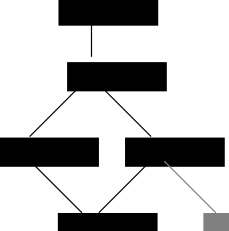
\includegraphics[width=0.35\textwidth]{pictures/hirarchy}
 \caption{Vererbungshierarchie für die Klasse Pokemon.}
 \label{hirarchy}
\end{figure}

Die Klasse Thing soll eine einfache Basisklasse sein und uns die Möglichkeit geben, die Syntax der Klassendefinition beider Ansätze zu vergleichen. Da Thing ledigleich eine leere Klasse ist, wollen wir im Anschluss zwei Klassen erstellen, deren Felder und Methoden später vererbt werden können: Element und Animal. Anhand von Element betrachten wir dabei zunächst, wie Felder und Methoden definiert werden können. Anhand der Klasse Animal und ihrer Subklasse Pet können wir das Konzept der Vererbung veranschaulichen. Es wird dann mit der Klasse Pokemon gezeigt, welche Möglichkeiten der Mehrfachvererbung es gibt.

Zusätzlich soll für beide Objektsysteme geprüft werden, welche Möglichkeiten es gibt, Methoden einer Superklasse in einer Subklasse zu ergänzen. 
\section{Das Objektsystem von Racket: Onstage}
Als Grundlage für dieses Kapitel dient die Racket-Dokumentation\cite{racketguide-classes} und -Referenz\cite{racketref-classes} für Klassen und Objekte.

Racket ist eine Multipurpose-Sprache und erlaubt die Auswahl der Syntax auf Sprachebene. Eine einzelne Codezeile bestimmt die Sprache eines Moduls, also beispielsweise, ob die Funktionen vorgezogen ausgewertet werden (\texttt{\#lang racket}) oder verzögert (\texttt{\#lang lazy}). Da das Objektsystem in die Sprache Racket integiert ist, kann man es direkt in jedem Racket-Modul verwenden.

% \begin{lstlisting}
%  #lang racket
% \end{lstlisting}

Die wichtigsten Werkzeuge, die man als Programmierer in einer objektorientierten Sprache benötigt, sind die Definition von Klassen, Feldern und Funktionen, sowie die Erzeugung von Objekten. Auf diese soll deshalb im Folgenden kurz eingegangen werden, bevor wir dazu kommen, welche Möglichkeiten es in Bezug auf Mehrfachvererbung im Objektsystem von Racket bereits gibt.

Alle Code-Beispiele sind auch noch einmal zusammenhängend in Anhang \ref{or-example} aufgeführt. 

\subsection{Einfache Klassen}

Eine Klasse wird in Racket durch das Schlüsselwort \texttt{class} definiert. Bei der Definition einer Klasse muss die Superklasse angegeben werden. Falls die Klasse keine (anderen) Superklassen hat, wird \texttt{object\%} angegeben, die eingebaute Rootklasse. Per Konvention enden Klassennamen in Racket auf \%, bei den folgenden Beispielen wird jedoch darauf verzichtet, um sie später leichter mit CLOS vergleichen zu können. Nach der Superklasse können noch beliebige Klassenoptionen, Felder oder Methoden definiert werden. An irgendeiner Stelle im Rumpf der Klasse muss jedoch mit \texttt{super-new} der Konstruktor der Oberklasse aufgerufen werden. Eine minimale Klassendefinition sieht damit folgendermaßen aus:

\begin{lstlisting}
(class object% (super-new))
\end{lstlisting}

Als Rückgabewert erhält man die Klasse\footnote{Streng genommen erhält man was anderes... TODO} %TODO
und kann sie für den späteren Zugriff in einer Variablen speichern. Die Variable wurde hier \texttt{thing} genannt.

\begin{lstlisting}
(define thing (class object% (super-new)))
\end{lstlisting}

Objekte von Klassen lassen sich mit dem Schlüsselwort \texttt{new} erzeugen:

\begin{lstlisting}
(new thing)
\end{lstlisting}

Felder lassen sich mit \texttt{init-field} oder \texttt{field} deklarieren, je nachdem, ob es möglich sein soll sie bei der Objekterzeugung zu initialisieren oder nicht. Für Methoden gibt es, je nach Art und Sichtbarkeit, unter anderem die Schlüsselwörter \texttt{define/public}, \texttt{define/private} und \texttt{define/override}. Die so definierten Methoden lassen sich anschließend mittels \texttt{send} aufrufen. Eine Element-Klasse, bestehend aus einem Feld für das Attribut und einem zugehörigen Getter- und Setter-Methode sieht beispielsweise folgendermaßen aus:

\begin{lstlisting}
(define element (class object% (super-new)
                  (init-field [attr 'water])
                  (define/public (get-attr) attr)
                  (define/public (set-attr value) (set! attr value))))  
\end{lstlisting}

Das Attribut (\texttt{attr}) kann bei der Initialisierung angegeben werden (es \emph{muss} angegeben werden, wenn kein Defaultwert spezifizert ist). Wird es nicht angegeben, enthält es standardmäßig den Wert \texttt{{\textquotesingle}water}. Mit den Methoden \texttt{get-attr} und \texttt{set-attr} können wir darauf zugreifen:

\begin{lstlisting}
(define elem (new element))

> elem
\end{lstlisting} 
{\routput (object:element ...)}

\begin{lstlisting}
> (send elem get-attr)
\end{lstlisting} 
{\rsymbol{water}}

\begin{lstlisting}
> (send elem set-attr 'wind)
> (send elem get-attr)
\end{lstlisting} 
{\rsymbol{wind}}

\begin{lstlisting}
(define elem2 (new element [attr 'fire]))

> (send elem2 get-attr)
\end{lstlisting} 
{\rsymbol{fire}}

Wir können uns auch eine Klasse Animal definieren, die von Thing erbt (auch wenn es nicht viel zu vererben gibt):

\begin{lstlisting}
(define animal (class thing (super-new)
                 (init-field [gender 'male]
                             [size 'small])
                 (define/public (get-gender) gender)
                 (define/public (get-size) size)))
\end{lstlisting} 

Und eine Klasse, die wiederum von Animal erbt:

\begin{lstlisting}
(define pet (class animal (super-new)
              (init-field [name 'unknown])
              (define/public (get-name) name)))
\end{lstlisting} 

Objekte der Klasse Pet besitzen dann alle drei Attribute:

\begin{lstlisting}
(define harry (new pet [name 'harry] [size 'normal]))

> (send harry get-name)
\end{lstlisting} 
{\rsymbol harry}

\begin{lstlisting}
> (send harry get-gender)
\end{lstlisting} 
{\rsymbol male}

\begin{lstlisting}
> (send harry get-size)
\end{lstlisting} 
{\rsymbol normal}

% TODO The make-object procedure creates a new object with by-position initialization arguments, the new form creates a new object with by-name initialization arguments, and the instantiate form creates a new object with both by-position and by-name initialization arguments.

Und das soll für diesen Zweck genügen. (Bis Manu sich in die Implementation eingelesen hat zumindest). %TODO

\subsection{Mehrfachvererbung in Racket}
Zuvor wurde behauptet, mit Racket könne man keine Mehrfachvererbung modellieren. Das ist nicht hundertprozentig richtig, denn tatsächlich gibt es zwei Arten von Klassen in Racket, die etwas ähnliches tun: Mixins und Traits. Es werden deshalb beide kurz vorgestellt, um aufzuzeigen, welche Probleme und Grenzen sie haben.

Dafür verwenden wir unsere vorher definierten Klassen Element und Animal. Beide haben unterschiedliche Felder und Methoden. Wir wollen versuchen, die Felder und Methoden aus beiden in einer neuen Klasse namens Pokemon zu vereinigen. Das ginge natürlich ganz simpel, indem eine der beiden Klassen in Pokemon umbenannt wird und von der anderen erbt, deshalb wollen wir außerdem fordern, dass beide Klassen auch einzeln verwendet können, sie sollen also nichts voneinaner wissen. 

\subsection{Mixins}
Da Klassen in Racket lediglich Ausdrücke sind, ist es möglich, sie als Parameter an Funktionen oder andere Klassen zu übergeben oder auch als Rückgabewert eines Funktionsaufruf zu definieren. Wir könnten uns beispielsweise eine Methode \texttt{generate-subclass} definieren, die eine Klasse als Parameter erhält und eine Subklasse von dieser erzeugt. Dafür muss sie den Parameter nur als Superklasse in einer Klassendefinition verwenden:

\begin{lstlisting}
(define (generate-subclass superclass)
  (class superclass (super-new)))
\end{lstlisting} 

Das ist noch keine sonderlich spannende Subklasse, da sie sich genauso verhält wie die angegebene Superklasse, aber wir können uns von ihrer Funktionalität überzeugen. Nehmen wir beispielsweise eine Subklasse der Klasse Element:

\begin{lstlisting}
> (generate-subclass element) 
\end{lstlisting}
{\routput \#<class:...>}

Dann erhalten wir das gleiche Verhalten wie für Objekte der Klasse Element:

\begin{lstlisting}
> (new (generate-subclass element))
\end{lstlisting}
{\routput (object:...)}

\begin{lstlisting}
> (send (new (generate-subclass element)) get-attr)
\end{lstlisting}
{\rsymbol water}

Nun könnte man in der in \texttt{generate-} \texttt{subclass} definierten Klasse natürlich auch noch weitere Felder und Methoden hinzufügen. Die Klasse fügt dann Verhalten zu einer bestehenden, aber noch unbekannten Klasse hinzu. Erst beim Methodenaufruf wird der Platzhalter mit einer tatsächlichen Superklasse gefüllt. Eine solche Klasse wird Mixin genannt und als Platzhalter für die Superklasse wird per Konvention \texttt{\%} genommen:

\begin{lstlisting}
(define (a-mixin %)
  (class % (super-new)
    ; neues Verhalten
    ))
\end{lstlisting}

Falls wir das Verhalten beider Klassen Element und Animal vereinen wollen, so könnten wir also eine von ihnen, oder beide, als Mixin definieren. Beide Klassen als Mixin zu definieren kommt am nächsten an unsere Idee von Mehrfachvererbung:

\begin{lstlisting}
(define (element-mixin %)
  (class % (super-new)
    (init-field [attr 'water])
    (define/public (get-attr) attr)))

(define (animal-mixin %)
  (class % (super-new)
    (init-field [gender 'male]
                [size 'small])
    (define/public (get-gender) gender)
    (define/public (get-size) size)))
\end{lstlisting}

Und aus diesen könnten wir uns dann alle drei Klassen Element, Animal und Pokemon erzeugen:
\begin{lstlisting}
(define element (element-mixin thing))

(define animal (animal-mixin thing))
 
(define pokemon (element-mixin (animal-mixin thing)))
\end{lstlisting}

Es wird Thing als Superklasse verwendet, da sie zuvor als leere Klasse definiert wurde. Genausogut hätten wir natürlich \texttt{object\%} benutzen können. Es fällt auf, dass die zwei Mixins nicht gleichwertig sind; wir müssen uns entscheiden, welches von beiden wir zuerst anwenden. Genau genommen passiert hier auch keine Mehrfachvererbung, sondern zweifache Einfachvererbung -- mit dem Vorteil jedoch, dass sich die zwei Klassen nicht kennen müssen und wir sie daher unabhängig voneinander verwenden können. Die Hierarchie sieht also wie folgt aus:

\texttt{pokemon $\rightarrow$ element $\rightarrow$ animal $\rightarrow$ thing $\rightarrow$ object\%}

Element und Animal verhalten sich genauso wie zuvor:

\begin{lstlisting}
> (send (new element [attr 'fire]) get-attr)
\end{lstlisting} 
{\rsymbol{fire}}

\begin{lstlisting}
> (send (new animal [size 'huge] [gender 'female]) get-size)
\end{lstlisting} 
{\rsymbol{huge}}

Zusätzlich können wir uns nun auch ein Pokemon definieren, das alle drei Eigenschaften aufweist:
\begin{lstlisting}
(define p (new pokemon [size 'large]
                       [gender 'female]
                       [attr 'fire]))
 
> (send p get-size)
\end{lstlisting}
{\rsymbol{large}}
\begin{lstlisting}
> (send p get-gender)
\end{lstlisting}
{\rsymbol{female}}
\begin{lstlisting}
> (send p get-attr)
\end{lstlisting}
{\rsymbol{fire}}

Falls es einen also nicht stört, für jede Klasse, die für Mehrfachvererbung in Frage kommt, zunächst eine Mixin-Klasse zu definieren und dass technisch eigentlich keine Mehrfachvererbung geschieht, so scheinen sich Mixins zunächst gut zur Modellierung zu eignen. Einen Umstand haben wir jedoch bisher außen vor gelassen: gleichbenannte Felder und Methoden. Element und Animal besitzen bisher eine disjunkte Menge von Feldern und Methoden. Das soll sich ändern. Nehmen wir an, es gibt eine Funktion \texttt{attack}, die sowohl Element als auch Animal haben. Ein Angriff des Elements Feuer soll einfach Feuer sein, bei Tieren sagen wir, der Angriff ist proportional zur Größe und auf Pokemon trifft beides zu. Der Einfachheit halber gibt die Funktion für Element und Animal also einfach die Werte der Felder \texttt{attr} und \texttt{size} zurück:

\begin{lstlisting}
(define (element-mixin %)
  (class % (super-new)
    (init-field [attr 'water])
    (define/public (get-attr) attr)
    (define/public (attack) attr))) ; neu
 
(define (animal-mixin %)
  (class % (super-new)
    (init-field [gender 'male]
                [size 'small])
    (define/public (get-gender) gender)
    (define/public (get-size) size)
    (define/public (attack) size))) ; neu
\end{lstlisting}

Nun schlägt jedoch die Definition der Klasse Pokemon fehl:

\begin{lstlisting}
> (define pokemon (element-mixin (animal-mixin thing)))
\end{lstlisting}
{\rerror $\bigotimes$ class*: superclass already contains method\\
method name: attack}

Racket erlaubt es nicht, dass zwei Methoden in einer Klasse den gleichen Namen haben. Wir dürfen geerbte Methoden aus Superklassen nicht neu deklarieren. Falls wir vorhaben, sie zu überschreiben, so müssen wir \texttt{define/override} verwenden:

\begin{lstlisting}
(define (element-mixin %)
  (class % (super-new)
    (init-field [attr 'water])
    (define/public (get-attr) attr)
    (define/override (attack) attr))) ; !
\end{lstlisting}

Das führt jedoch dazu, dass wir nun bei der Erstellung der Element-Klasse nicht mehr \texttt{thing} als Superklasse angeben können, denn die Klasse Thing bietet keine Funktion \texttt{attack}, die überschrieben werden könnte. Wollen wir also weiterhin, dass es möglich ist, sich Objekte von der Klasse Element zu erzeugen, so müssen wir eine Klasse bereitstellen, die eine solche Methode anbietet, damit Element von ihr erben kann.

\begin{lstlisting}
(define element (element-mixin (class object% 
                                       (super-new)
                                       (define/public (attack) null))))
\end{lstlisting}

Zudem ist der Angriff einer Pokemons nun ledlichlich der Wert des Feldes \texttt{attr}. Für unser Pokemon \texttt{p} von oben ergibt das:
\begin{lstlisting}
> (send p attack)
\end{lstlisting}
{\rsymbol fire}

Was wir eigentlich wollen, ist jedoch eine Kombination aus der Größe und dem Element. Das heißt, damit Pokemon das gewünschte Verhalten zeigt, müsste Element eine Kombination aus dem eigenen Wert und dem der Superklasse zurückgeben.

\begin{lstlisting}
(define (element-mixin %)
  (class % (super-new)
    (init-field [attr 'water])
    (define/public (get-attr) attr)
    (define/override (attack) (list (super attack) attr)))) ; !
\end{lstlisting}

Abgesehen davon, dass es nicht sehr guter Programmierstil ist, die Logik der Klasse Pokemon in eine andere Klasse auszulagern, hat es wiederum Einfluss auf Objekte der Klasse Element. Anstatt des Attributs erhält man nun eine etwas seltsam anmutende Liste:

\begin{lstlisting}
> (send (new element) attack)
\end{lstlisting}
{\rsymbol (() water)}

Dafür zeigt Pokemon nun das gewünschte Verhalten.
\begin{lstlisting}
> (send p attack)
\end{lstlisting}
{\rsymbol (large fire)}

Es ist jedoch nicht mehr möglich, die Reihenfolge der Mixins zu vertauschen. Eine Definition von Pokemon als

\begin{lstlisting}
(define pokemon (animal-mixin (element-mixin thing)))
\end{lstlisting}

führt zu einem Fehler, aus dem gleichen Grund wie vorher bei Objekten der Klasse Element: da Element eine Superklasse erwartet, die eine Funktion \texttt{attack} anbietet. Da Thing nun die direkte Superklasse ist, ist das nicht mehr der Fall. Selbst wenn wir das beheben würden, würde die Erzeugung nun an Animal hängen bleiben, da es die geerbte Methode aus Element nicht überschreibt, sondern versucht neu zu definieren. Wir müssten alle Schritte, die wir soeben zur erfolgreichen Vererbung von der Methode \texttt{attack} durchgeführt haben, für den umgekehrten Fall definieren. Wollen wir beide Vererbungs-Reihenfolgen erlauben, wird zudem die Funktion \texttt{attack} deutlich komplizierter, da nun anhand der Superklasse entschieden werden müsste, ob der Wert des Feldes direkt zurückgegeben werden kann oder eine Kombination mit dem Wert der Superklasse nötig ist.

Wir haben zudem bisher nur zwei Superklassen betrachtet. Bei drei, vier oder gar 20 Superklassen, die vielleicht selbst wiederum von mehreren Superklassen erben, wird, falls eine sinnvolle Modellierung mit Mixins überhaupt noch möglich ist, der Code extrem unübersichtlich und schwer wartbar. Insbesondere für die Lehre von Mehrfachvererbung eignen sie sich demnach nicht.

\subsection{Traits}
Traits sind ähnlich zu Mixins. Sie kapseln eine Menge von Methoden, die zu einer Klasse hinzugefügt werden sollen. Traits erlauben jedoch Kontrolle darüber, welche Methoden wie geerbt werden. Es ist möglich bestimmte Methoden nicht zu erben, sie unter einem Alias zu erben oder mit Trait-Operatoren zu manipulieren und die Ergebnisse mehrerer Methoden zu kombinieren.

Sie lösen damit eines der fundamentalen Probleme von Mixins: Die Vererbung und Kombination gleichbenannter Methoden. Wenn es in zwei Traits, die kombiniert werden sollen, gleichbenannte Methoden gibt, so hat der Programmierer die Möglichkeit (und Pflicht), anzugeben, wie diese Kollision gelöst werden soll, üblicherweise durch Ausschließen oder Umbenennen einer der Methoden in der Subklasse, oder durch Methodenkombination.

Die Definition von Traits ist syntaktisch fast identisch zu der Definition einer Klasse, es gibt nur zwei Unterschiede: Anstelle des Schlüssworts \texttt{class} wird \texttt{trait} benutzt und es müssen weder Superklasse noch Superkonstruktor-Aufrug angegeben werden. Traits unterstützen einen Großteil der Optionen, die auch \texttt{class} unterstützt, unter anderem aber keine \texttt{init-field}s. Was das für unser Beispiel bedeutet, sehen wir gleich. Prinzipiell können wir jedoch unsere Defintion für Element und Animal fast eins zu eins übernehmen. 

\begin{lstlisting}
(require racket/trait)

(define element-trait
  (trait (field [attr 'water]) ; statt init-field
         (define/public (get-attr) attr)
         (define/public (attack) attr)))

(define animal-trait
  (trait (field [gender 'male] ; statt init-field
                [size 'small])
         (define/public (get-gender) gender)
         (define/public (get-size) size)
         (define/public (attack) size)))
\end{lstlisting}

Wenn wir ein Pokemon-Trait aus diesen beiden Traits definieren wollen, müssen wir den Konflikt der beiden \texttt{attack}-Methoden beheben. Das geht jedoch, im Gegensatz zu Mixins direkt im Pokemon-Trait. Zur Manipulation der Vererbung gibt verschiedene Trait-Operationen, wie
\begin{itemize}
 \item \texttt{trait-exclude}, das eine Methode von einem Trait entfernt,
 \item \texttt{trait-alias}, welches die Kopie einer Methode unter anderem Namen zum Trait hinzufügt und
 \item \texttt{trait-sum}, welche die Methoden von zwei Traits kombiniert.
\end{itemize}

Das Vorgehen bei einem Konflikt lässt sich generalisieren. Zunächst wird dafür gesorgt, dass es keinen Namenskonflikt mehr gibt. Dafür wird aus den zwei Traits mit kollidierender Methode jeweils ein neuer Trait erstellt, in dem diese Methode einen neuen, eindeutigen Namen erhält. Dafür würden wir beispielweise zum Trait Element mit \texttt{trait-alias} einen Alias für die \texttt{attack}-Methode hinzufügen, den wir \texttt{element-attack} nennen. Der Trait hat anschließend \emph{zwei} Funktionen für den Angriff, \texttt{attack} und \texttt{element-attack}, die beide das gleiche tun. Anschließend können wir mit \texttt{trait-exclude} die ursprüngliche \texttt{attack}-Methode von der Vererbung ausschließen. Es wird also nur die Alias-Methode \texttt{element-attack} vererbt.

Dieser Schritt wird für jeden Konflikt durchgeführt. Sobald alle Methoden einen eindeutigen Namen haben, können sie dann mit \texttt{trait-sum} kombiniert werden.

\begin{lstlisting}
 (define pokemon-trait
   (trait-sum   ; Kombiniere die folgenden Traits
    (trait-exclude (trait-alias element-trait   ; Erstelle Alias fuer
                                attack          ; attack und entferne
                                element-attack) ; das Original
                   attack)
    (trait-exclude (trait-alias animal-trait    ; Analog fuer animal
                                attack         
                                animal-attack)
                   attack)
    (trait (inherit element-attack animal-attack) ; Kombiniere die zwei
           (define/public (attack)                ; attack-Methoden
             (list (animal-attack) (element-attack))))))
\end{lstlisting}

Wir erhalten einen neuen Trait. 

\begin{lstlisting}
> pokemon-trait
\end{lstlisting}
{\routput \#<trait>}

Man kann Traits nicht direkt zu Klassen hinzufügen, aber man kann sie mit der Funktion \texttt{trait->mixin} in ein Mixin umwandeln und dieses dann zu einer Klasse hinzufügen:

\begin{lstlisting}
 (define pokemon ((trait->mixin pokemon-trait) thing))
\end{lstlisting}

Ich muss noch herausfinden, wie man die Felder dann initialisiert. Man kann zwar per Hand init schreiben, aber dann sind keine optionalen Parameter mehr möglich. %TODO

Hier abschließender Satz zu Problemen mit Object-Racket. %TODO

%------------------------------------------------------------------------------------------------

\section{CLOS: Onstage}
Grundlage für dieses Kapitel ist das Buch ``Object-Oriented Programming in Common Lisp. A Programmer's Guide to CLOS''\cite{keene} von Sonya E. Keene. 

Das Common Lisp Object System ist der Standard für objektorientierte Programmierung in der Sprache Common Lisp. Auch Racket bietet es an, in diesem Stil objektorientiert zu programmieren. Um anstatt des Racket-Objektsystems mit CLOS-Objekten zu arbeiten, muss lediglich die Sprache auf Swindle umgestellt werden:


\begin{lstlisting}
#lang swindle
\end{lstlisting}

Wir wollen nun versuchen, die Klassen Thing, Element, Animal und Pokemon auch in CLOS zu schreiben, um zu sehen, welche Unterschiede in der Syntax es gibt und wie Mehrfachvererbung hier umgesetzt ist. 

Alle Code-Beispiele sind auch noch einmal zusammenhängend in Anhang \ref{clos-example} aufgeführt.

\subsection{Einfache Klassen}
Für die Definition von Klassen in CLOS gibt es das Makro \texttt{defclass}. Im Gegensatz zu dem Objektsystem von Racket erstellt das Makro eine benannte Klasse. Der Name wird beim Aufruf mit übergeben und damit erübrigt sich eine anschließende Benennung mit \texttt{define}. Auch in CLOS wird die Superklasse mit angegeben. Da es jedoch mehrere Superklassen geben kann, werden diese in einer Liste übergeben. Hat die Klasse keine Superklassen (außer der Rootklasse), so wird die leere Liste übergeben. Die explizite Angabe der Rootklasse als Superklasse nicht nicht nötig. Anschließend können noch die Slots der Klasse angegeben werden, aber für eine minimale Klasse ohne Superklasse(n) genügt der Name und die leere Liste: 

\begin{lstlisting}
((defclass thing ())
\end{lstlisting}

% Zur Objekterzeugung gibt es in CLOS zwei verschiedene Möglichkeiten, je nachdem ob \texttt{:automaker} als Klassen-Option gesetzt wurde oder nicht. 

Objekte dieser Klasse können mit dem Schlüsselwort \texttt{make} erzeugt werden.

\begin{lstlisting}
> (make thing)
\end{lstlisting}
{\routput \#thing}

Felder oder Slots, wie sie in CLOS üblicherweise genannt werden, werden nach der Superklasse angegeben. Ein großer Unterschied zu dem Objektsystem von Racket ist, dass innerhalb einer Klassendefinition \textit{nur} Slots definiert werden, keine Methoden. Methoden werden außerhalb der Klasse definiert. Wie genau das aussieht, sehen wir gleich. Zunächst sorgt dieser Umstand jedoch dafür, dass kein Schlüsselwort benötigt wird, um anzugeben, ob gerade ein Slot oder eine Methode definiert wird. Wir könnten also, für die Definition der Klasse Element beispielweise, einfach schreiben:

\begin{lstlisting}
(defclass element (thing)
  attr)
\end{lstlisting}

Die Klasse hat genau einen Slot namens \texttt{attr}, der jedoch so noch nicht sehr nützlich ist.

Damit mit diesem Slot auch interargiert werden kann, benötigt er noch Accessoren: einen Getter (in CLOS Reader genannt) und einen Setter (in CLOS Writer genannt). Außerdem möchte man gegebenenfalls einen Initialwert angeben können, den Slot dokumentieren und so weiter. All dies geschieht durch Slot-Optionen. Sie folgen nach dem Namen des Slots (der nun geklammert werden muss, damit klar ist, wann die Slot-Definition zuende ist) und beginnen mit einem Doppelpunkt. Um auf das Attribut \texttt{attr} beispielsweise lesend oder schreibend zugreifen zu können, kann die Slot-Option \texttt{:reader} oder \texttt{writer} gesetzt werden oder, falls beides möglich sein soll und man Code-Zeilen sparen will, auch die Option \texttt{:accessor}. Accessoren müssen benannt werden. Im Gegensatz zu dem Objektsystem von Racket muss sich der Name jedoch nicht vom Namen des Slots unterscheiden. Hier also die vollständige Definition der Klasse:

\begin{lstlisting}
(defclass element (thing)
  (attr
    :accessor attr
    :initvalue 'water
    :initarg :attr))
\end{lstlisting}

Zusätzlich zu den Accessoren wurde auch noch ein Initialwert definiert und ein Schlüsselwort, mit dem er bei der Objekterzeugung angegeben werden kann. Die Namen der Accessoren können direkt wie Methoden genutzt werden:

\begin{lstlisting}
> (attr (make element))
\end{lstlisting}
{\routput water}

\begin{lstlisting}
> (attr (make element :attr 'fire))
\end{lstlisting}
{\routput fire}

Der Wert kann dann nach der Objekterzeugung mittels \texttt{set!} verändert werden:

\begin{lstlisting}
(define elem (make element))
> (attr elem)
\end{lstlisting}
{\routput water}

\begin{lstlisting}
> (set! (attr elem) 'wind)
> (attr elem)
\end{lstlisting}
{\routput wind}

Um für die Abfrage des Zustands eines Objektes nicht immer alle sondierenden Methoden aufrufen zu müssen, bietet CLOS die Klassen-Option \texttt{:printer}, die bewirkt, dass bei Auswertung des Objektes ein formattierter String ausgegeben wird. Wir fügen es zu unserer Element-Klasse hinzu.

\begin{lstlisting}
(defclass element (thing)
  (attr
    :accessor attr
    :initvalue 'water
    :initarg :attr)
  :printer #t) ; auf Klassenebene
\end{lstlisting}

Wenn wir jetzt ein Objekt erzeugen, oder das Auswertungsergebnis eines bereits erzeugten Objektes abfragen, so erhalten wir sofort auch die Belegung aller Slots:

\begin{lstlisting}
> (make element)
\end{lstlisting}

{\routput \#<element: attr=water>}

Falls wir oft die Slots mit Werten initialisieren, so kann die Option \texttt{:automaker} gesetzt werden.

\begin{lstlisting}
(defclass element (thing)
  (attr
    :accessor attr
    :initvalue 'water
    :initarg :attr)
  :printer #t
  :automaker #t) ; auf Klassenebene
\end{lstlisting}

Sie bewirkt, dass sich die Syntax bei der Objekterzeugung verkürzt. Anstatt zu jedem Slot, der initialisiert wird, den Namen angeben zu müssen, können wir die Werte direkt nacheinander auflisten. Falls es mehrere Slots gibt, muss die Parameterreihenfolge mit der Reihenfolge der Slots in der Klassendeifnition übereinstimmen. Statt

\begin{lstlisting}
(make element :attr 'fire)
\end{lstlisting}

können wir nun verkürzt schreiben:

\begin{lstlisting}
(make-element 'fire)
\end{lstlisting}

Zusätzlich zu dem Schlüsselwort \texttt{make} zur Erzeugung von allgemeinen Objekten gibt es nun das Schlüsselwort \texttt{make-element} zur Erzeugung von Objekten der Klasse Element. Element-Objekte können natürlich auch weiterhin mit \texttt{make} erzeugt werden.

Falls eine Klasse viele Slots hat und die Accessoren für alle Slots gleich dem Slot-Namen sein sollen, so kann man als Klassenoption \texttt{:autoaccessors} auf \texttt{:slot} setzen. Damit sparen wir uns beispiesweise bei der Definition der Klasse Animal, die zwei Slots für Geschlecht und Größe hat, eine Code-Zeile. Wenn wir zusätzlich \texttt{:automaker} benutzen, kann auch die \texttt{:initarg}-Option  weggelassen werden\footnote{Das hat natürlich zur Folge, dass nun bei der Objekterzeugung mit \texttt{make} die Slots nicht mehr initialisiert werden können.}.

\begin{lstlisting}
(defclass animal (thing)
  (gender :initvalue 'male)
  (size   :initvalue 'small)
  :autoaccessors :slot
  :automaker #t
  :printer #t)
\end{lstlisting}



\begin{lstlisting}
---------------------------------------------

(print (make-animal))
(printf "~n")
(print (make-animal 'female 'medium))
(printf "~n")

(defclass pokemon (animal element)
  (index :initvalue 0
         :type <number>)
  :autoaccessors :slot
  :automaker #t
  :printer #t)

(define p1 (make-pokemon))
(print p1)
(printf "~n")
(define p2 (make-pokemon 'fire 'female 'large 42))
(print p2)
(printf "~n")

(defgeneric attack ((t thing))
  :combination generic-list-combination)

(defmethod attack ((e element))
  (attr e))

(defmethod attack ((a animal))
  (size a))

(print (attack p1))
(printf "~n")
(print (attack p2))
\end{lstlisting}

\section{Zwischen-Fazit}

\section{CLOS: Backstage}

% 
% \chapter{Entwurf?}
% https://docs.racket-lang.org/drracket/extending-drracket.html
% \chapter{Implementation}
% \chapter{Zusammenfassung und Ausblick}

% -----------------------------------------------------------------------------------------

\appendix
\chapter{Anhang}
\section{Beispiel Object-Racket}
\label{or-example}
\lstinputlisting{code/object-racket-example.rkt}

\section{Beispiel CLOS}
\label{clos-example}
\lstinputlisting{code/clos-example.rkt}

\cleardoublepage
\phantomsection % benötigt für korrekte pdf-darstellung
\addcontentsline{toc}{chapter}{Literaturverzeichnis}
\bibliographystyle{alpha} % originally: natbib % Din 1505 nach Lorenzen (Das konkrete Aussehen des Litverzeichnisses ist im header festgelegt)
% \bibliography{bibliography/literatur}  % Pfad zur *.bib-Datei (Dateiendung wird weggelassen)
%TODO korrekt zitieren
Werden noch korrekt zitiert und ggf. durch bessere Quellen ersetzt. 
\begin{thebibliography}{}
 \bibitem{amop} The Art of the Metaobject Protocol 
 \bibitem{racketguide-dialects} \url{http://docs.racket-lang.org/guide/dialects.html}
 \bibitem{neu-edu} \url{http://www.ccs.neu.edu/home/matthias/Thoughts/Programming\_with\_Class\_in\_Racket.html}
 \bibitem{neu-edu2} \url{http://www.ccs.neu.edu/home/matthias/Tmp/Class/programming-with-class/Classes\_in\_Racket.html}
 \bibitem{racketguide-classes} Racket Guide: 13. Classes and Objects \url{https://docs.racket-lang.org/guide/classes.html}
 \bibitem{racketref-classes} Racket Reference: 6. Classes and Objects \url{https://docs.racket-lang.org/reference/mzlib\_class.html}
 \bibitem{racketguide-macros} \url{https://docs.racket-lang.org/guide/macros.html}
 \bibitem{racketref-macros} \url{https://docs.racket-lang.org/reference/Macros.html}
 \bibitem{fearofmacros} \url{http://www.greghendershott.com/fear-of-macros/index.html}
 \bibitem{keene} Sonya E. Keene, ``Object-Oriented Programming in Common Lisp. A Programmer's Guide to CLOS''
\end{thebibliography}

\cleardoublepage % TODO
\backmatter 

\thispagestyle{empty}

\vspace*{\fill}
\pagestyle{empty}

{\normalsize
\begin{center}\textbf{Eidesstattliche Erklärung}\end{center}
Hiermit versichere ich an Eides statt, dass ich die vorliegende Arbeit im Masterstudiengang Informatik selbstständig verfasst und keine anderen als die angegebenen Hilfsmittel – insbesondere keine im Quellenverzeichnis nicht benannten Internet-Quellen – benutzt habe. Alle Stellen, die wörtlich oder sinngemäß aus Veröffentlichungen entnommen wurden, sind als solche kenntlich gemacht. Ich versichere weiterhin, dass ich die Arbeit vorher nicht in einem anderen Prüfungsverfahren eingereicht habe und die eingereichte schriftliche Fassung der auf dem elektronischen Speichermedium entspricht.
\vspace*{1cm}\\
Hamburg, den XX.XX.20XX
\hspace*{\fill}\begin{tabular}{@{}l@{}}\hline
\makebox[5cm]{Vorname Nachname}
\end{tabular}
\vspace*{3cm}
%Dies ist optional, ggf. löschen!
\begin{center}\textbf{Veröffentlichung}\end{center}
Ich stimme der Einstellung der Arbeit in die Bibliothek des Fachbereichs Informatik zu.
\vspace*{1cm}\\
Hamburg, den XX.XX.20XX
\hspace*{\fill}\begin{tabular}{@{}l@{}}\hline
\makebox[5cm]{Vorname Nachname}
\end{tabular}
}
\vspace*{\fill} 

\end{document}
